% Evangelos 2009/12/19

\subsection{\label{s:mfReqb}\CLe\  general \slice}

As became clear in \refsect{s:cleCoordSlice}, the use of a coordinate \slice\ \refeq{cLeCoordSlice}
allowed explicit determination of invariant variable \refeq{eq:invLaser} and straightforward
determination of invariant variables \refeq{eq:invLaser}. Unfortunately the moving frame
method introduced artificial singularities in \reducedsp, that as we've seen in \refsect{sec:CLeMovFr}
depends on the choice of slice point.
% On the other hand \slice\ \refeq{cLeCoordSlice} is defined to be orthogonal
% to the group tangent of \SOn{2} restricted in the $x$-irreducible subspace of \SOn{2}
% and this introduces singularities in the transformations \refeq{eq:invLaser}.
Therefore we examine in this section a different choice of slice fixing point that appears natural.
% In hope to remove these singularities, in this section we construct a moving frame
Since \REQB{1} organizes reduced space dynamics around it but also sets the
scale of angular velocity of symmetry induced rotations in the system, we
pick $\slicep=\ssp_{\REQB{1}}$ as the slice fixing point.
The price to pay is that it won't be convenient to explicitly write out
transformations to invariant variables
as we did in \refsect{sec:mf}; we will instead implement the moving frame map numerically,
mapping computed trajectories to the \slice.
This is by no means a drawback. Even though computation of invariants with the
{\mframes} is efficient, it is still
prohibitive for very high dimensional flows. For, one has
to compute the invariants with computer algebra, a proccess
that works\rf{SiminosThesis} for moderate system dimension of the order of $100$,
as required for instance in truncations of \KSe\ studied in \refref{SCD07},
but does not scale well for problems with truncations of order $10,000$ as
a fully resolved $3$-D fluid simulation would easily require\rf{GibsonPhD}.
\ES{dropped: We will demonstrate in the example of \cLe\
how one can use the geometric interpretation of the {\mframes}
to simply and effectively, perform continuous symmetry
reduction in high-dimensional flows.}


Choosing a point on \reqv\ group orbit,
$\slicep  = \ssp_{\REQB{1}}$,
each group intersects the section exactly twice,  with the
two solutions separated by $\pi$. We select the one \ESedit{
that is at the smallest Euclidean distance from $\slicep$}
\ES{replaced but not sure: with a
smaller clockwise rotation angle into the \slice.} or use
the explicit expression \refeq{cLeMF}.\ES{dropped
as I am not sure it is correct for multiparameter groups. Even
for \cLe\ it seems to imply that the slice exists on the $z$-axis,
which I think is not true: The
invariant subspaces are always within the \slice, as $\Lg_a
 \ssp =0$ for $\ssp$ in an invariant subspace.
}
Projections of \cLe\ dynamics to the slice defined in this way are
shown in \reffig{fig:CLEmfReqb1}. Eventhough less evident, singularities
of the same nature as the ones in \refsect{s:cLeCoordMF} are also present
here.


%%%%%%%%%%%%%%%%%%%%%%%%%%%%%%%%%%%%%%%%%%%%%%%%%%%%%%%%%%%%%%%%
%computed with vaggelis/testing/flows/CLEfinalTmp.nb
\begin{figure}[ht]
\begin{center}
  (\textit{a})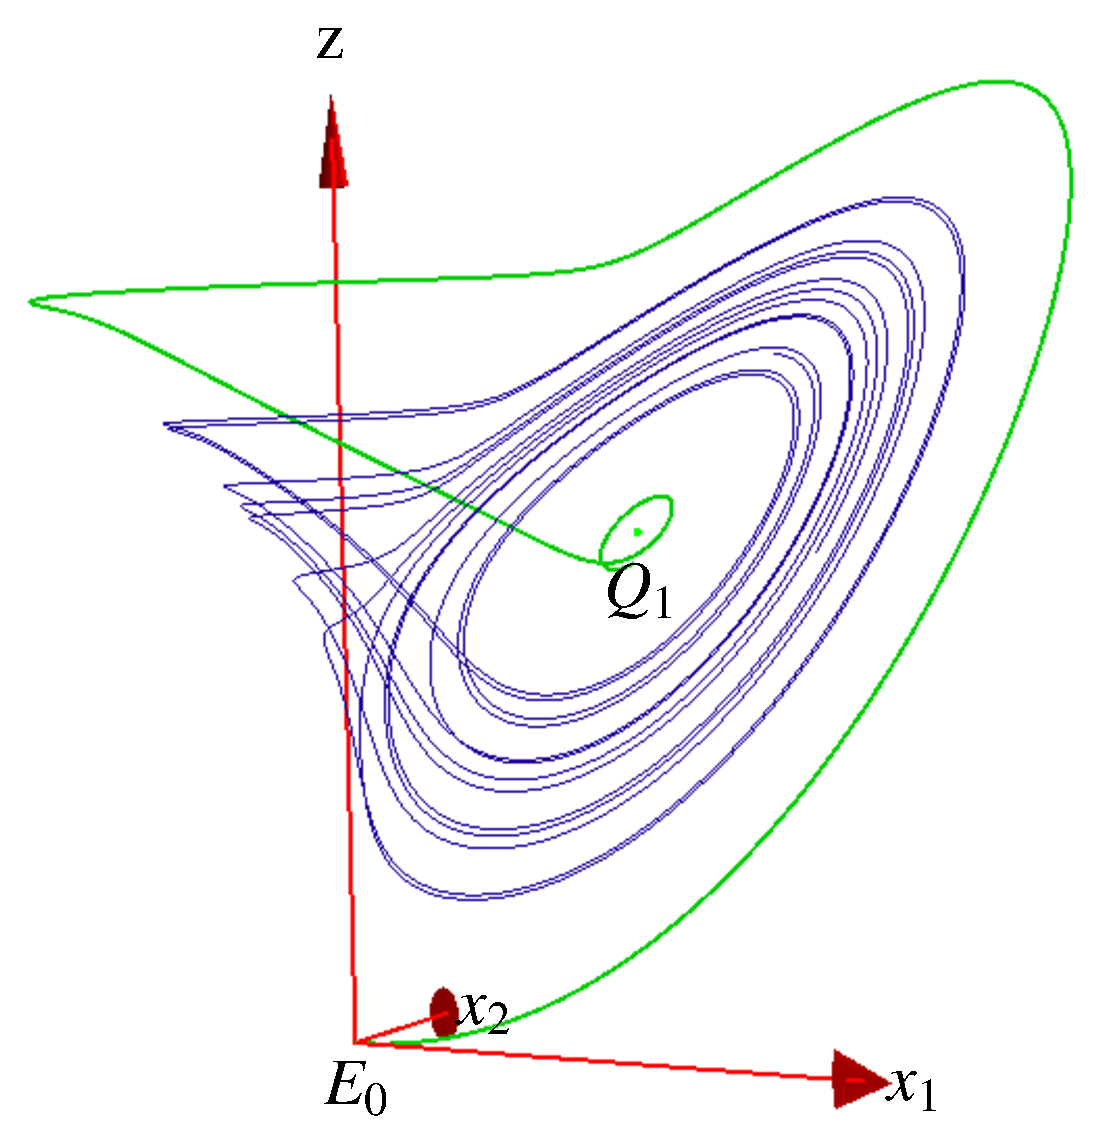
\includegraphics[width=0.35\textwidth,clip=true]{../figs/CLEmfReqb1}
~~~~(\textit{b})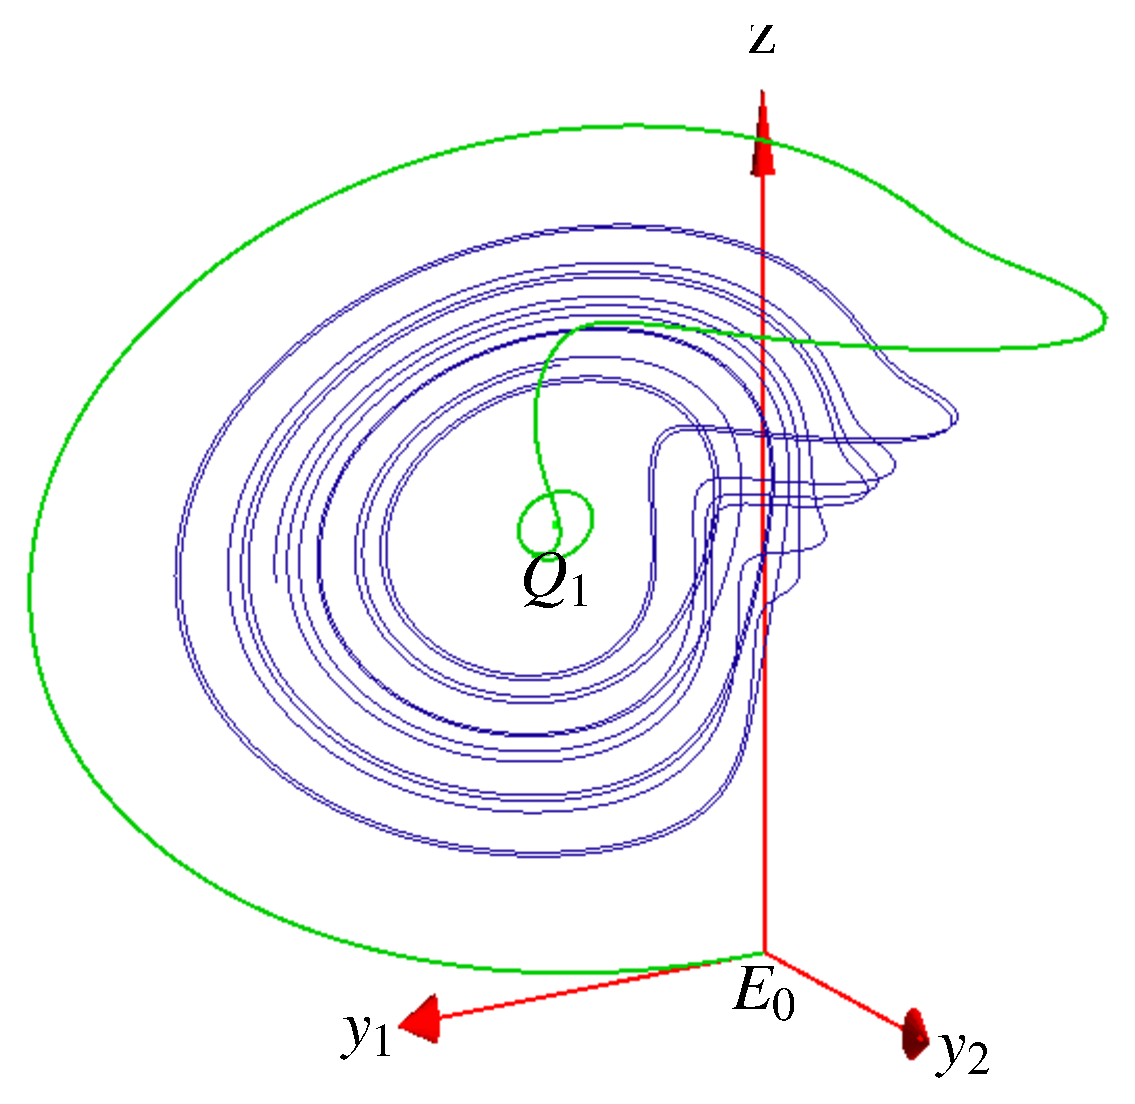
\includegraphics[width=0.35\textwidth,clip=true]{../figs/CLEmfReqb}
\end{center}
\caption{
\Statesp\ portraits of \cLe\ dynamics in \reducedsp. We use a
moving frame map to a slice orthogonal to the group tangent
at  $\slicep  = \ssp_{\REQB{1}}$. $x_2$ and $y_2$ rescaled
for clarity.
    }
\label{fig:CLEmfReqb1}
\end{figure}
%%%%%%%%%%%%%%%%%%%%%%%%%%%%%%%%%%%%%%%%%%%%%%%%%%%%%%%%%%%%%%%%

\PublicPrivate{}{
In \reffig{CLEmfDali}(a) we observe that with slice fixed by
$\slicep=\ssp_{\REQB{1}}$ the attractor meets the \sset\ head
on and becomes deformed. Choosing the slice fixing point as
$\slicep=\ssp_{\REQB{1}}+(0,-5,0,0,0)$ we can tilt the \sset\
so that trajectories approach it in a smoother manner, see
\reffig{fig:CLEmfDali}(b), \reffig{fig:CLEmfAdHoc}.
    \ES{Dali melting clock attractor}
%     \PC{in three figure captions,
%        \reffig{fig:CLEmfDali}, \reffig{fig:CLEmfAdHoc}
%        you mention rescaling $y_2$ `for clarity', but there
%        is no $y_2$ in figures.
%        }
%%%%%%%%%%%%%%%%%%%%%%%%%%%%%%%%%%%%%%%%%%%%%%%%%%%%%%%%%%%%%%%%
%computed with vaggelis/testing/flows/CLEfinalTmp.nb
\begin{figure}[ht] \label{fig:CLEmfDali}
\begin{center}
  (\textit{a})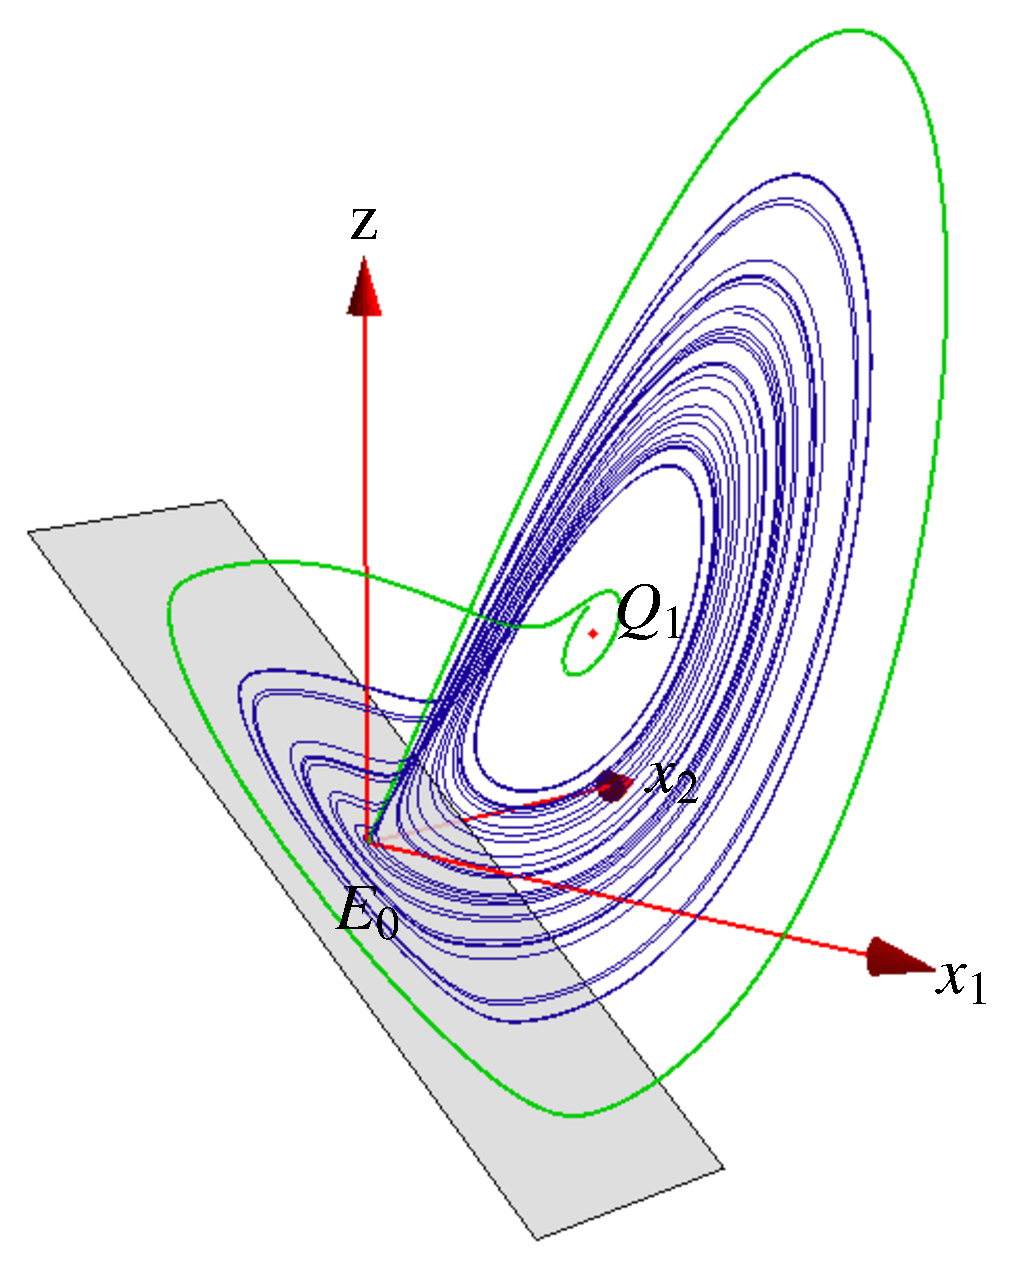
\includegraphics[width=0.35\textwidth,clip=true]{../figs/CLEmfReqb123}
~~~~(\textit{b})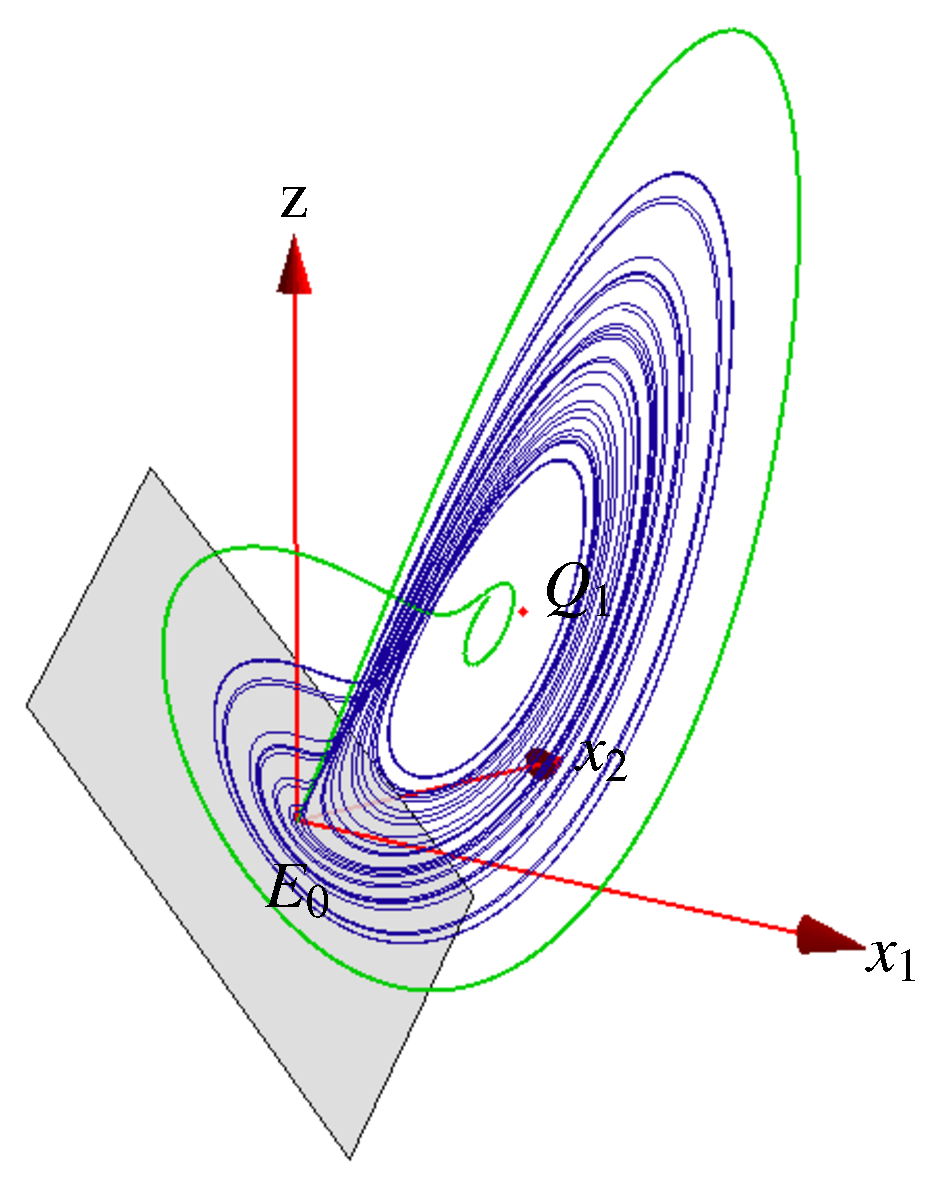
\includegraphics[width=0.35\textwidth,clip=true]{../figs/CLEmfAdHoc123}
\end{center}
\caption{
\Statesp\ portraits of \cLe\ dynamics in \reducedsp. We use a
moving frame map to a slice orthogonal to the group tangent
at  (a)$\slicep  = \ssp_{\REQB{1}}$, (b) $\slicep  =
\ssp_{\REQB{1}}+(0,-5,0,0,0)$. The gray plane indicates the \sset.
    }
\end{figure}
%%%%%%%%%%%%%%%%%%%%%%%%%%%%%%%%%%%%%%%%%%%%%%%%%%%%%%%%%%%%%%%%

%%%%%%%%%%%%%%%%%%%%%%%%%%%%%%%%%%%%%%%%%%%%%%%%%%%%%%%%%%%%%%%%
%computed with vaggelis/testing/flows/CLEfinalTmp.nb
\begin{figure}[ht]
\begin{center}
  (\textit{a})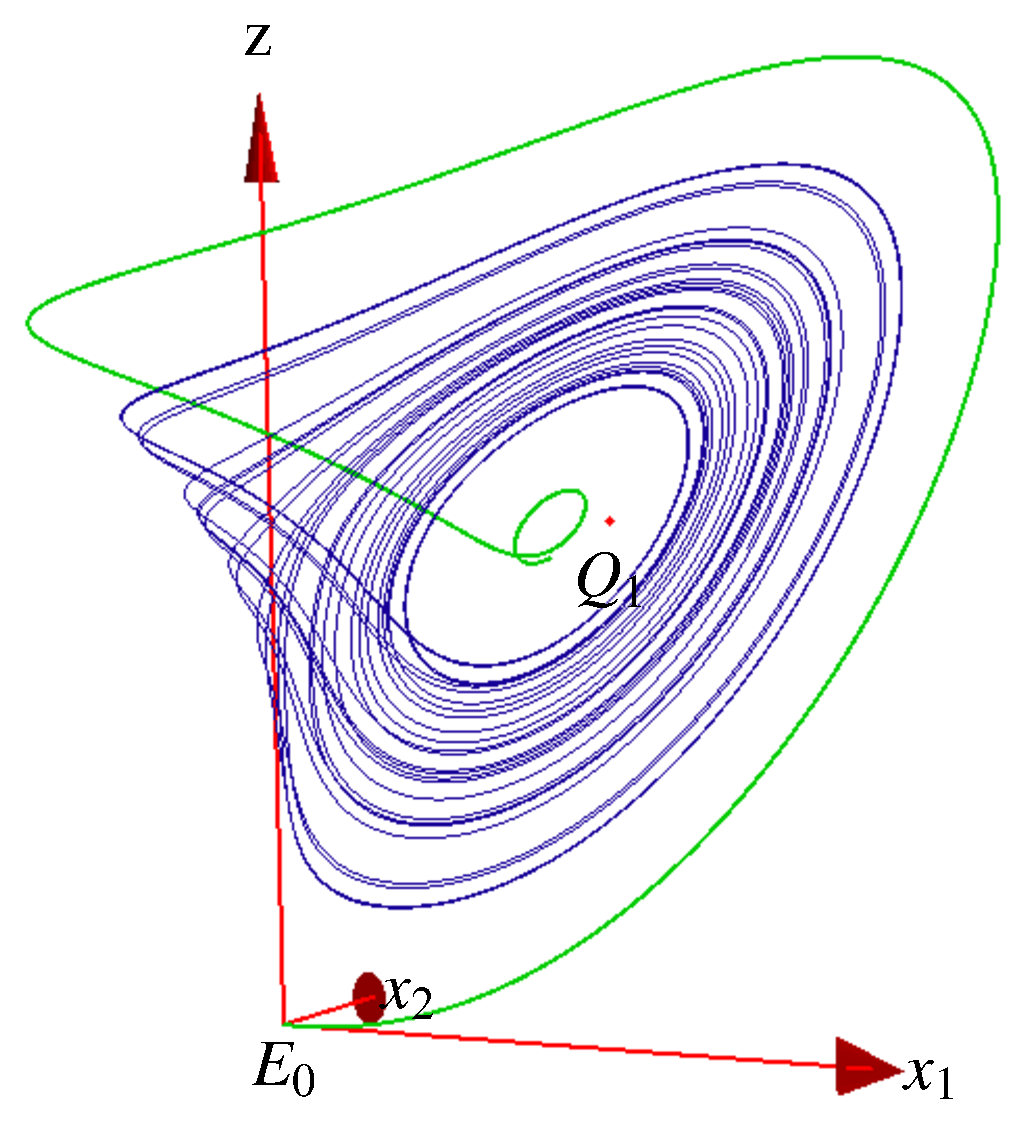
\includegraphics[width=0.35\textwidth,clip=true]{../figs/CLEmfAdHoc1}
~~~~(\textit{b})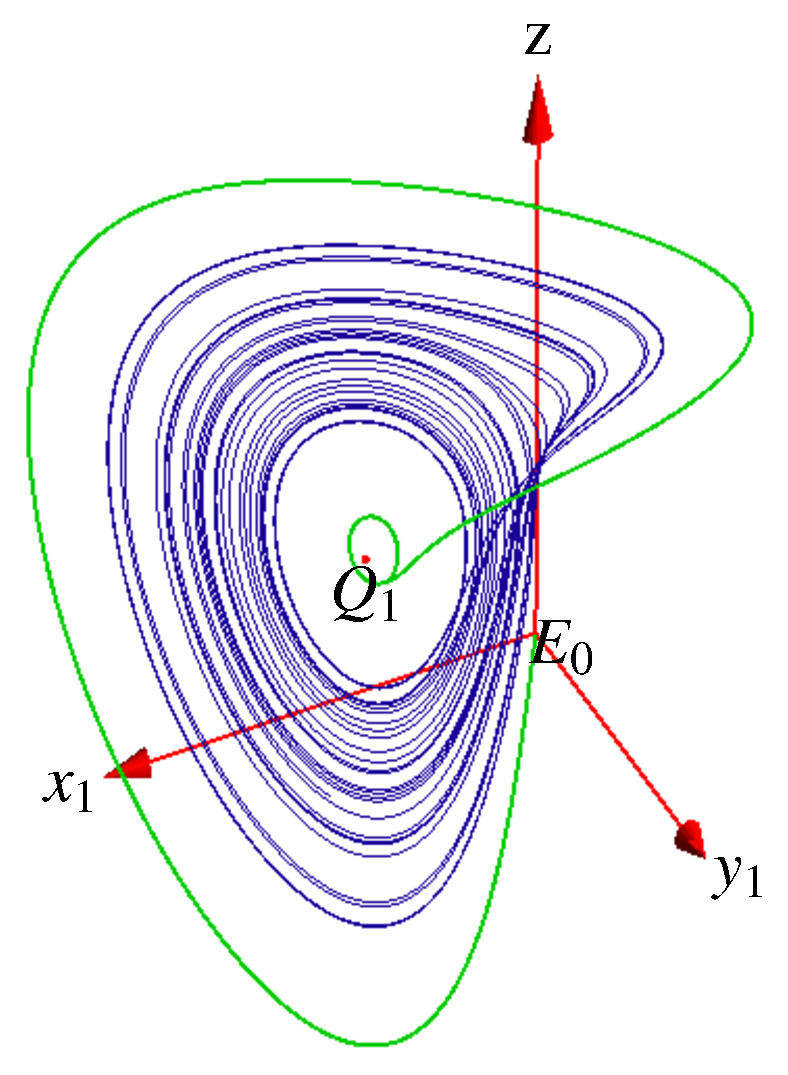
\includegraphics[width=0.35\textwidth,clip=true]{../figs/CLEmfAdHoc135}
\end{center}
\caption{
\Statesp\ portraits of \cLe\ dynamics in \reducedsp. We use a
moving frame map to a slice orthogonal to the group tangent
at $\slicep  = \ssp_{\REQB{1}}+(0,-5,0,0,0)$.
    }
\label{fig:CLEmfAdHoc}
\end{figure}
%%%%%%%%%%%%%%%%%%%%%%%%%%%%%%%%%%%%%%%%%%%%%%%%%%%%%%%%%%%%%%%%


}% end PublicPrivate


Rotation of $\ssp$ by angle $\theta$
to the slice defined by \refeq{PCsectQ1} is a linear operation
for any given point and can be applied efficiently
even in a high dimensional space. This is especially true
for truncations of PDEs, when typically the rotation group
representation is a direct sum of irreducible
representations and one is not force to store large matrices.
Of course, the transformation is still non-linear
through the dependence on the angle and equivalent to the
explicit transformations \refeq{eq:invLaser}.


Since rotations commute with time integration, one can take a
different approach: starting with a point on the slice
integrate for small but finite time and then map the
corresponding orbit segment to the section and repeat the
procedure. In this setting it is easier to distinguish
between the two points of intersection of the slice and the
group orbit (for instance we can peek the one with a smaller
clockwise rotation angle into the \slice) but we get no
further practical advantages. Nevertheless, in the limit of
infinitesimal time steps this procedure reveals the
connection of \mframes\ method to its continuous time
counterpart of \refsect{sec:MovFrameODE}.
    \ES{I didn't see the need to write a subsection for this.}
